\documentclass{article}

% Language setting
% Replace `english' with e.g. `spanish' to change the document language
\usepackage[english]{babel}

% Set page size and margins
% Replace `letterpaper' with `a4paper' for UK/EU standard size
\usepackage[letterpaper,top=2cm,bottom=2cm,left=3cm,right=3cm,marginparwidth=1.75cm]{geometry}

% Useful packages
\usepackage{amsmath}
\usepackage{graphicx}
\usepackage[colorlinks=true, allcolors=blue]{hyperref}

\title{PS 10}
\author{Haocheng Yang}

\begin{document}
\maketitle



\section{Comparison Among ML Methods}

Please see the attached two pictures that shows the prediction and performance for each machine learning model. As we can see, Neural Network could generate the highest estimate which is 0.92, and the logistic regression using roc auc metric generated a close result. All the estimates using roc auc metric show higher estimates than the estimate produced from accuracy metric. Overall, the Neural Network method relatively performs better than other methods. And the tree model performs relatively bad.


\begin{figure}
\centering
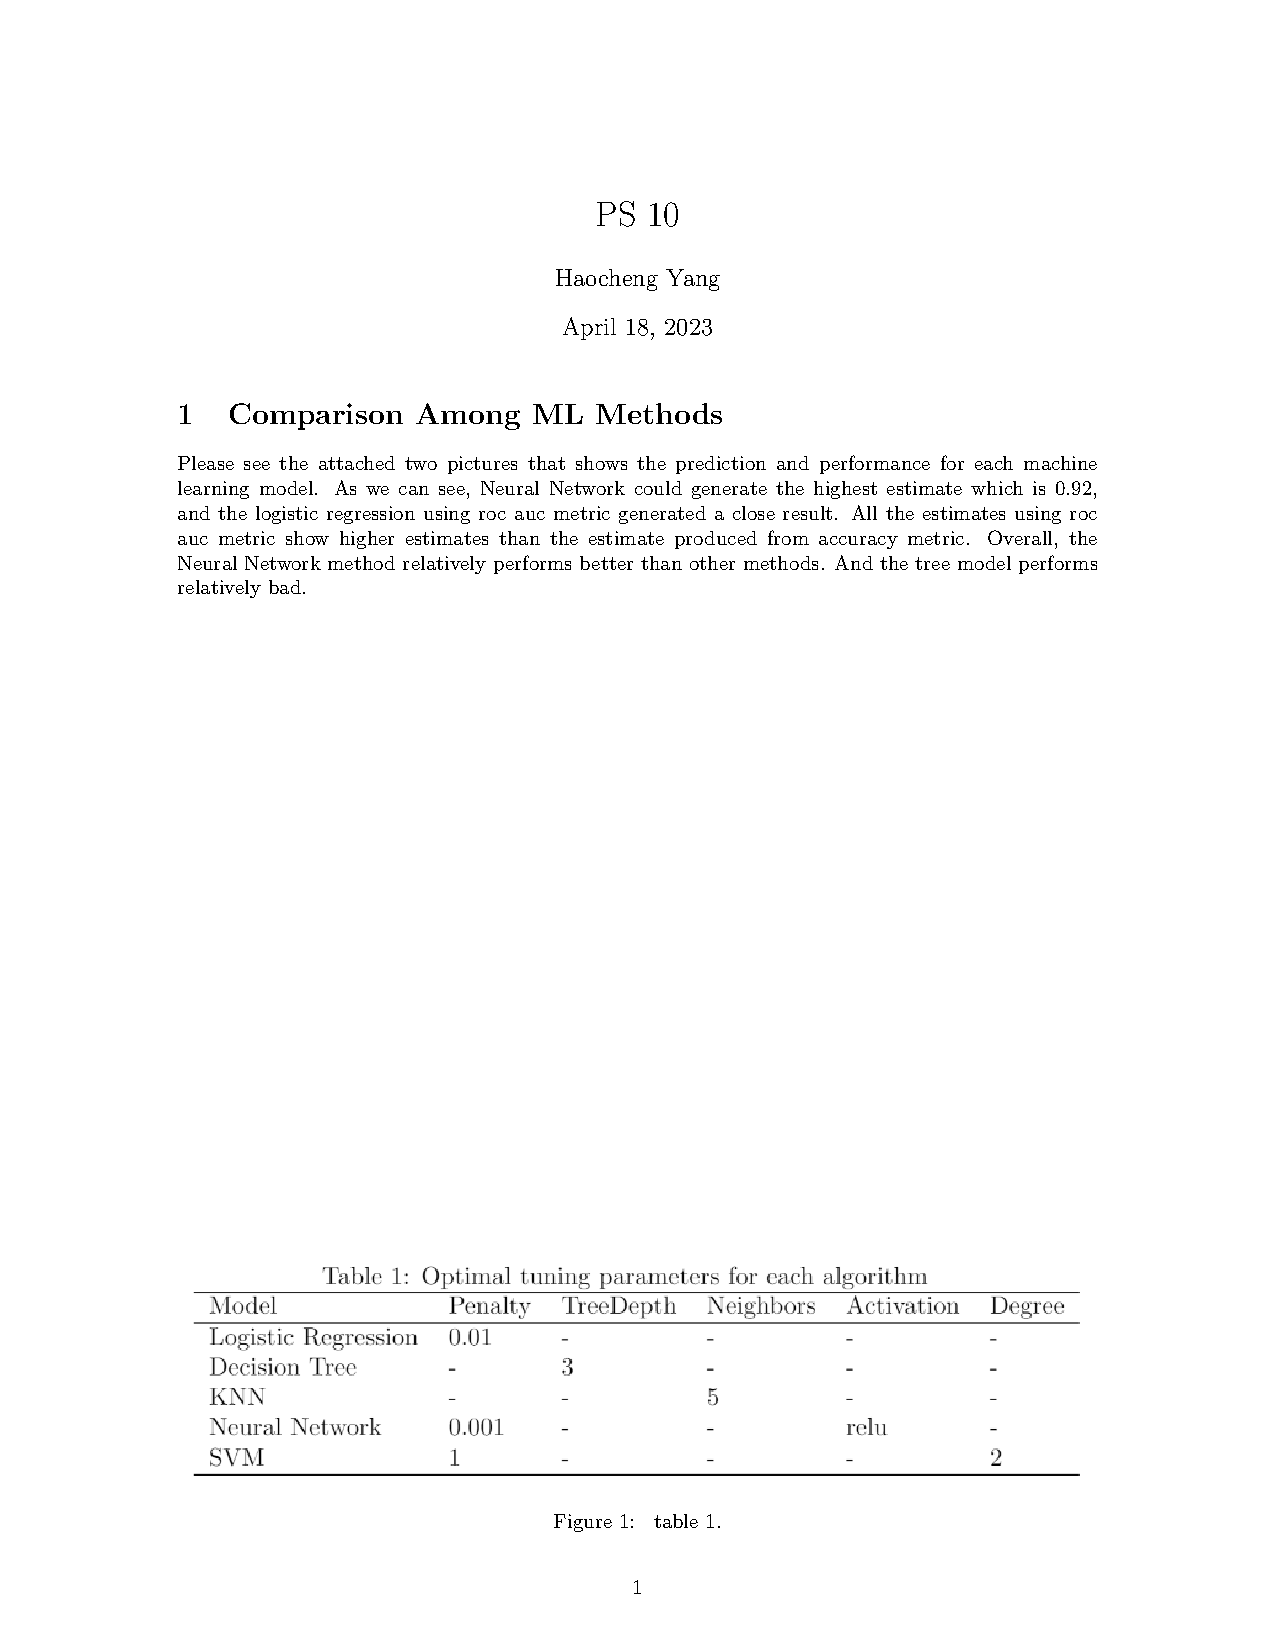
\includegraphics[width=1\textwidth]{PS10_Yang.png}
\caption{\label{fig:1} table 1.}
\end{figure}

\begin{figure}
\centering
\includegraphics[width=1\textwidth]{PS10.png}
\caption{\label{fig:1} table 2.}
\end{figure}



\end{document}